\part{Annexe}

\chapter{Photos illustratives d'équipements informatique}

\begin{figure}[H]
	\centering
	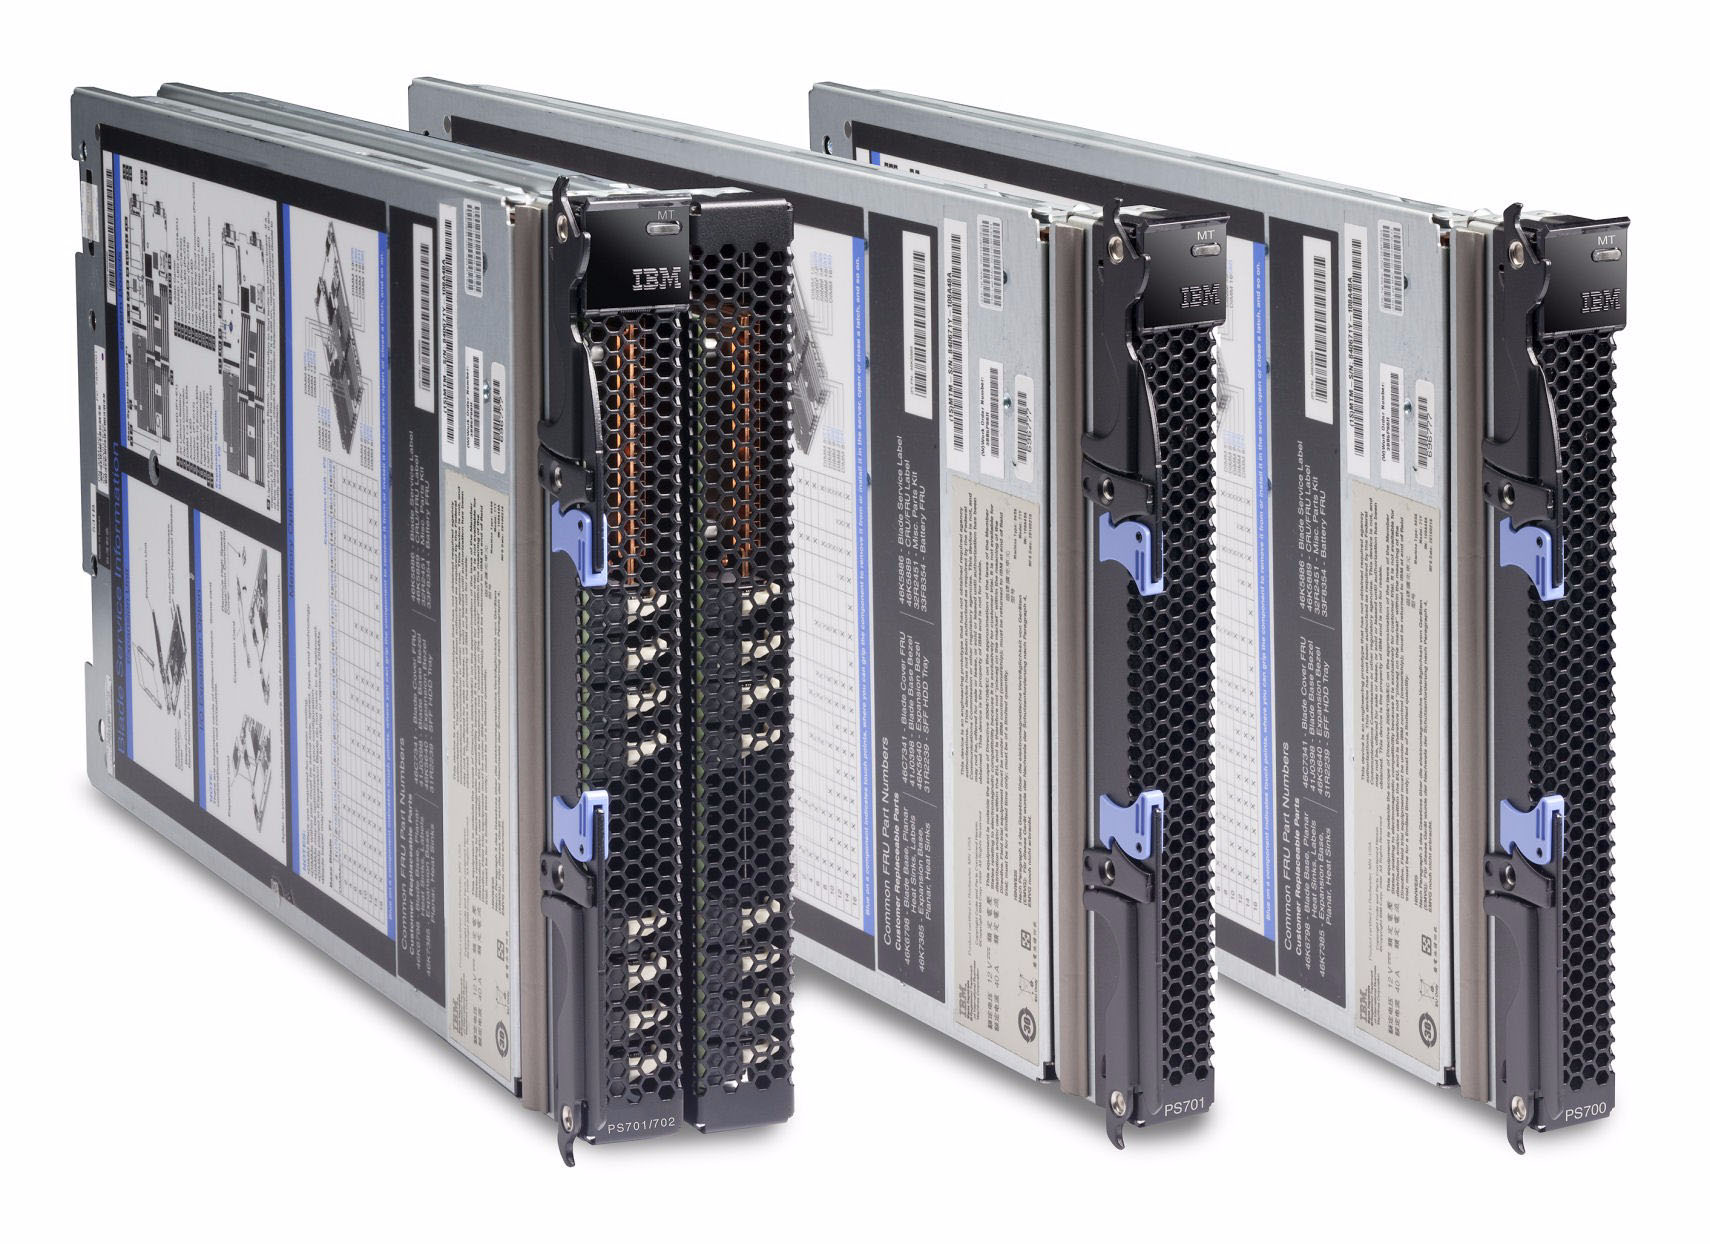
\includegraphics[width=0.6\textwidth]{resource/img/blade}
	\caption{Trois serveurs lames (\emph{blade server} en anglais)}
\end{figure}

\begin{figure}[H]
	\centering
	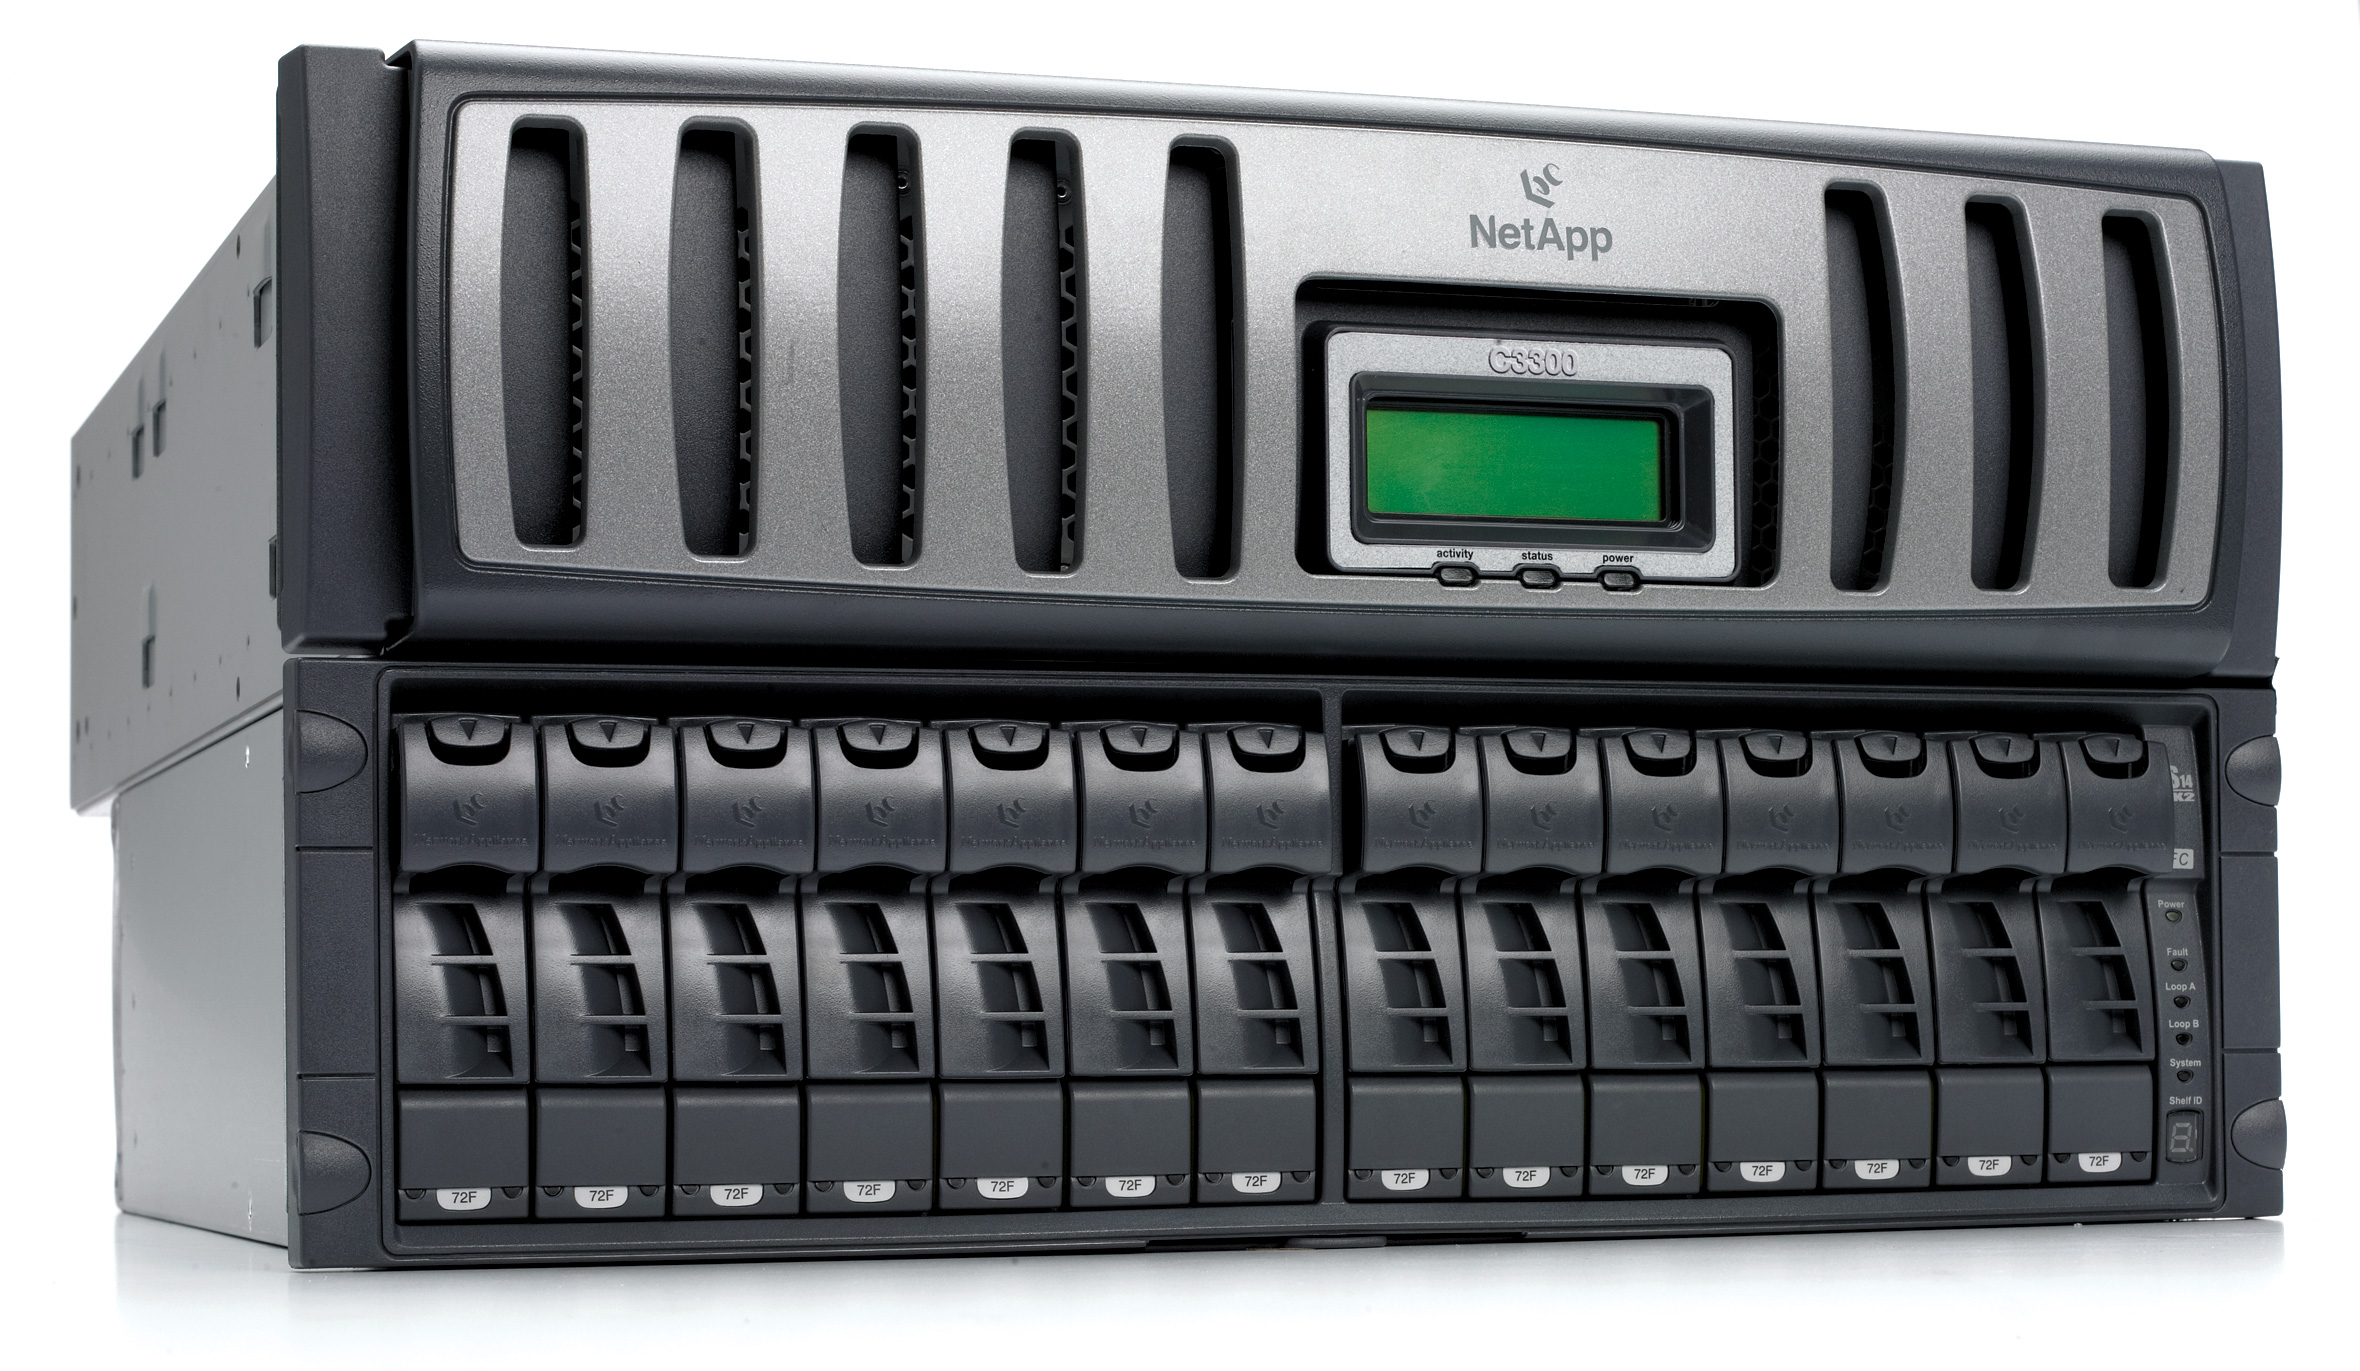
\includegraphics[width=0.6\textwidth]{resource/img/netapp_c3300}
	\caption{Baie de disque NetApp C3300 contenant 14 disques durs}
	\label{netapp}
\end{figure}

\begin{figure}[H]
	\centering
	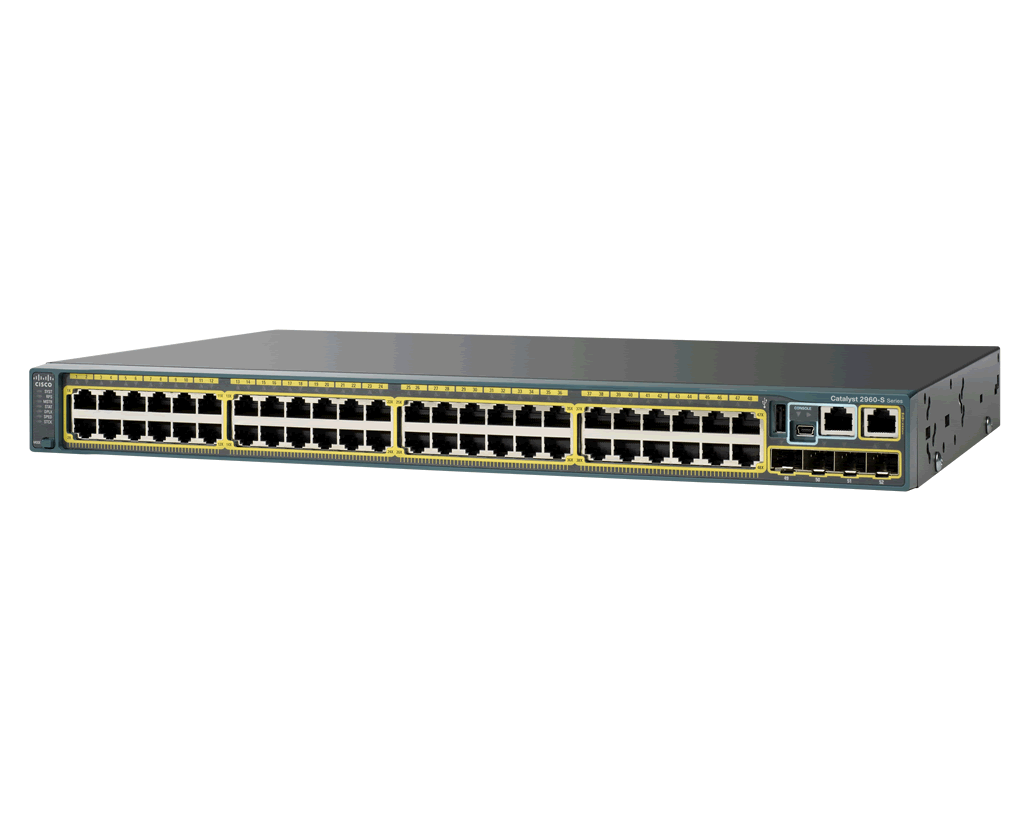
\includegraphics[width=0.6\textwidth]{resource/img/cisco-switch}
	\caption{Switch Cisco WS-C2960}
\end{figure}

\begin{figure}[H]
	\centering
	\includegraphics[width=0.6\textwidth]{resource/img/DC}
	\caption{Plusieurs baies de serveur (\emph{rack} en anglais) dans un Data Center}
	\label{datacenter}
\end{figure}

\chapter{Résumé des changement apportés à OpenNebula pour l'ajout de la gestion \emph{storage backend}}
\label{modopennebula}
\begin{lstlisting}
 SConstruct                                     |    6 +-
 include/AuthManager.h                          |    4 +-
 include/DispatchManager.h                      |   17 ++-
 include/Image.h                                |   18 ++-
 include/ImageManager.h                         |   30 ++--
 include/ImagePool.h                            |    2 +
 include/Nebula.h                               |   26 ++-
 include/RequestManagerAllocate.h               |   39 +++-
 include/RequestManagerDelete.h                 |   18 ++
 include/RequestManagerHost.h                   |   20 ++
 include/RequestManagerImage.h                  |   27 +++
 include/RequestManagerInfo.h                   |   18 ++
 include/RequestManagerPoolInfo.h               |   18 ++
 include/RequestManagerStorageBackend.h         |   59 +++++
 include/RequestManagerUpdateTemplate.h         |   18 ++
 include/StorageBackend.h                       |  184 +++++++++++++++
 include/StorageBackendPool.h                   |   85 +++++++
 include/StorageBackendTemplate.h               |   27 +++
 include/StorageManager.h                       |  155 ++++++++++++
 include/StorageManagerDriver.h                 |   53 +++++
 include/TransferManager.h                      |   46 +++--
 include/TransferManagerDriver.h                |   89 +++++++-
 include/VirtualMachine.h                       |   17 ++-
 install.sh                                     |   34 +++-
 share/etc/oned.conf                            |   33 +++-
 share/man/SConstruct                           |    1 -
 src/acct/watch_helper.rb                       |    6 +-
 src/cli/etc/oneimage.yaml                      |    5 +
 src/cli/etc/onestoragebackend.yaml             |   50 ++++
 src/cli/one_helper.rb                          |    2 +-
 src/cli/one_helper/oneimage_helper.rb          |    8 +-
 src/cli/one_helper/onestoragebackend_helper.rb |  110 +++++++++
 src/cli/oneimage                               |   21 ++
 src/cli/onestoragebackend                      |   98 ++++++++
 src/cloud/common/CloudAuth/EC2CloudAuth.rb     |    2 -
 src/cloud/common/CloudAuth/X509CloudAuth.rb    |    3 +-
 src/dm/DispatchManagerActions.cc               |   47 ++++
 src/image/Image.cc                             |   26 ++-
 src/image/ImageManagerActions.cc               |    6 +
 src/image/ImageManagerDriver.cc                |    1 +
 src/image/ImagePool.cc                         |   37 ++-
 src/lcm/LifeCycleActions.cc                    |    1 +
 src/lcm/LifeCycleStates.cc                     |    2 -
 src/mad/MadManager.cc                          |    1 +
 src/mad/ruby/ActionManager.rb                  |   20 +-
 src/mad/ruby/StorageDriver.rb                  |  101 ++++++++
 src/mad/ruby/TransfertManagerDriver.rb         |  170 ++++++++++++++
 src/nebula/Nebula.cc                           |   31 +++-
 src/nebula/SConstruct                          |    2 +
 src/oca/ruby/OpenNebula.rb                     |    2 +
 src/oca/ruby/OpenNebula/Image.rb               |   12 +-
 src/oca/ruby/OpenNebula/Pool.rb                |   11 +-
 src/oca/ruby/OpenNebula/StorageBackend.rb      |  127 ++++++++++
 src/oca/ruby/OpenNebula/StorageBackendPool.rb  |   53 +++++
 src/oca/ruby/OpenNebula/XMLUtils.rb            |    1 -
 src/onedb/onedb                                |    6 +-
 src/onedb/onedb_backend.rb                     |   18 +-
 src/rm/Request.cc                              |    2 +
 src/rm/RequestManager.cc                       |   24 ++-
 src/rm/RequestManagerAllocate.cc               |   16 ++
 src/rm/RequestManagerImage.cc                  |   88 +++++++
 src/rm/RequestManagerStorageBackend.cc         |   69 ++++++
 src/rm/RequestManagerVirtualMachine.cc         |   18 ++-
 src/rm/SConstruct                              |    1 +
 src/sm/SConstruct                              |   12 +
 src/sm/StorageManager.cc                       |  298 ++++++++++++++++++++++++
 src/sm/StorageManagerDriver.cc                 |  228 ++++++++++++++++++
 src/sm_mad/dummy/one_sm_dummy                  |   37 +++
 src/sm_mad/dummy/one_sm_dummy.rb               |   42 ++++
 src/storagebackend/SConstruct                  |   12 +
 src/storagebackend/StorageBackend.cc           |  256 ++++++++++++++++++++
 src/storagebackend/StorageBackendPool.cc       |   87 +++++++
 src/storagebackend/test/SConstruct             |    1 +
 src/test/Nebula.cc                             |    1 +
 src/tm/TransferManager.cc                      |  131 ++++++-----
 src/tm/TransferManagerDriver.cc                |  156 ++++++++++++-
 src/tm_mad/dummy/one_tm_dummy                  |   37 +++
 src/tm_mad/dummy/one_tm_dummy.rb               |   43 ++++
 src/tm_mad/dummy/tm_dummy.conf                 |   23 --
 src/tm_mad/dummy/tm_dummy.sh                   |   19 --
 src/tm_mad/dummy/tm_dummyrc                    |   15 --
 src/tm_mad/lvm/tm_context.sh                   |    9 +-
 src/tm_mad/lvm/tm_lvmrc                        |    3 -
 src/tm_mad/shared/tm_context.sh                |   10 +-
 src/tm_mad/shared/tm_sharedrc                  |    4 -
 src/tm_mad/ssh/tm_context.sh                   |   10 +-
 src/tm_mad/ssh/tm_mv.sh                        |   17 +-
 src/tm_mad/ssh/tm_sshrc                        |    4 -
 src/tm_mad/tm_common.sh                        |   14 --
 src/vm/VirtualMachine.cc                       |    4 +
 src/vm/VirtualMachinePool.cc                   |   55 +++++
 91 files changed, 3471 insertions(+), 299 deletions(-)
\end{lstlisting}

\chapter{H2O}

\section{Résumé du code développé}

\begin{lstlisting}
 bin/h2o-archive            |  181 +++++++++++++
 bin/h2o-block              |  392 +++++++++++++++++++++++++++
 bin/h2o-cluster            |  598 +++++++++++++++++++++++++++++++++++++++++
 bin/h2o-loader             |  186 +++++++++++++
 bin/h2o-setup-db           |   22 ++
 bin/h2o-vif                |  235 ++++++++++++++++
 bin/h2o-vm                 |  529 ++++++++++++++++++++++++++++++++++++
 bin/h2ocheck               |  143 ++++++++++
 bin/h2od                   |   94 +++++++
 conf.rb                    |   11 +
 lib/cli.rb                 |  332 +++++++++++++++++++++++
 lib/dm-options.rb          |   35 +++
 lib/errors.rb              |   16 ++
 lib/lockable.rb            |   16 ++
 lib/logging.rb             |   11 +
 lib/manageable.rb          |  185 +++++++++++++
 lib/manager.rb             |   52 ++++
 lib/modules.rb             |    5 +
 lib/sshtarget.rb           |  109 ++++++++
 lib/tagable.rb             |   64 +++++
 managers/archive.rb        |   84 ++++++
 managers/block-pool.rb     |  130 +++++++++
 managers/block.rb          |  142 ++++++++++
 managers/cluster.rb        |   53 ++++
 managers/hypervisor.rb     |   94 +++++++
 managers/loader.rb         |   41 +++
 managers/vif.rb            |   99 +++++++
 managers/vm.rb             |  640 +++++++++++++++++++++++++++++++++++++++++++
 model/vm.rb                |  642 ++++++++++++++++++++++++++++++++++++++++++++
 modules/dummyblockpool.rb  |   66 +++++
 modules/dummyhypervisor.rb |   42 +++
 modules/netapp.rb          |  379 ++++++++++++++++++++++++++
 modules/xenhypervisor.rb   |  397 +++++++++++++++++++++++++++
 remote/attach-block.sh     |    3 +
 remote/pack.sh             |   23 ++
 remote/unpack.sh           |   31 +++
 templates/xmdomain.erb     |   21 ++
 tests/check.sh             |   52 ++++
 tests/cleanup-netapp.sh    |   10 +
 tests/dropshell.sh         |    4 +
 tests/reset-archivepool.sh |    4 +
 tests/reset-hyp.sh         |   10 +
 tests/reset-master.sh      |    4 +
 tests/reset-netapp.sh      |   12 +
 tests/vm-lifecycle.sh      |   59 ++++
 45 files changed, 6258 insertions(+), 0 deletions(-)
\end{lstlisting}

\section{La \emph{Command Line Interface}}
\label{CLIH2O}
\subsection{Interface de gestion de cluster}

\begin{lstlisting}
paulg@debian-pro:~/projects/h2o$ ./bin/h2o-cluster list
=>Argument Error<=
The first argument must be an action


Possible actions:
        register-hyp <cluster-id> <driver> <hostname> <ssh-user> <ssh-host>
        register-blockpool <cluster-id> <driver> <name> <target-ip> <management-ip> <management-user>
        register-cluster <name> <archive_pool_ip> <archive_pool_user>
        list-hyp [--cluster <id>] [--show-destroyed]
        list-blockpool [--cluster <id>] [--show-destroyed]
        list-cluster [--show-destroyed]
        unregister-hyp <id>
        unregister-blockpool <id>
        unregister-cluster <id>
        lock-cluster <id>
        lock-hyp <id>
        lock-blockpool <id>
        unlock-cluster <id>
        unlock-hyp <id>
        unlock-blockpool <id>
        unload-hypervisor <id>
        clear-error-cluster <id>
        clear-error-hyp <id>
        clear-error-blockpool <id>
        retry-cluster <id>
        retry-hyp <id>
        retry-blockpool <id>
        set-tag-hyp <id> [[+|-]<tag> ...]
        set-tag-blockpool <id> [[+|-]<tag> ...]
        show-hyp <id>
        show-blockpool <id>

Global optional arguments
        --raw : Print results formated for easy scripting
        --override: Disable most checks when trying to do the action
        --force: Will try harder to do the action
        --wait: Wait for the action to finish before returning
\end{lstlisting}

\subsection{Interface de gestion de VMs}

\begin{lstlisting}
paulg@debian-pro:~/projects/h2o$ ./bin/h2o-vm
=>Argument Error<=
The first argument must be an action


Possible actions:
        create <clusterId> <name>
        destroy <id>
        start <id>
        halt <id>
        reboot <id>
        mem-set <id> <size> #The memory size is in megabytes
        maxmem-set <id> <size> #The max memory size is in megabytes
        vcpu-set <id> <vcpu count>
        maxvcpu-set <id> <max vcpu count>
        show <id>
        list [--cluster <clusterId>] [--hyp <hypId>] [--show-destroyed]
        livemigrate <id> <hypervisorId>
        attach-block <id> <blockId>
        detach-block <id> <blockId>
        attach-vif <id> <vifId>
        detach-vif <id> <vifId>
        #create-if <vmId> <mac> <vlan> [--ip]... [--bandwidth] #TODO
        #destroy-if <vmId> <mac> #TODO
        pin <mvId> <hypervisorId>
        unpin <vmId>
        lock <id>
        unlock <id>
        clear-error <id>
        retry <id>
        set-tag <id> [[+|-]<tag> ...]

Global optional arguments
        --raw : Print results formated for easy scripting
        --override: Disable most checks when trying to do the action
        --force: Will try harder to do the action
        --wait: Wait for the action to finish before returning
\end{lstlisting}

\subsection{Interface de gestion des images disques (appelés blocks)}

\begin{lstlisting}
paulg@debian-pro:~/projects/h2o$ ./bin/h2o-block
=>Argument Error<=
The first argument must be an action


Possible actions:
        allocate <clusterId> <name> <size>
        clone <name> <parentBlockId>
        unpack <archiveId> <blockName> <size> <fsType:fsOptions>
        pack <blockId> <archiveName>
        deploy <id>
        list [--cluster <id>] [--show-destroyed]
        destroy <id>
        resize <id> <newSize> #The new size is in MB
        volatile <id>
        persistant <id>
        lock <id>
        unlock <id>
        clear-error <id>
        retry <id>
        set-tag <id> [[+|-]<tag> ...]

Global optional arguments
        --raw : Print results formated for easy scripting
        --override: Disable most checks when trying to do the action
        --force: Will try harder to do the action
        --wait: Wait for the action to finish before returning
\end{lstlisting}

\subsection{Interface de gestion des archives d'OS}

\begin{lstlisting}
paulg@debian-pro:~/projects/h2o$ ./bin/h2o-archive
=>Argument Error<=
The first argument must be an action


Possible actions:
        list [--cluster <id>] [--show-destroyed]
        show <id>
        upload <clusterId> <archiveName> <uri>
        (download <archiveId> <uri>)
        destroy <id>
        rename <archiveId> <newArchiveName>

Global optional arguments
        --raw : Print results formated for easy scripting
        --override: Disable most checks when trying to do the action
        --force: Will try harder to do the action
        --wait: Wait for the action to finish before returning
\end{lstlisting}

\chapter{Benchmark des I/Os disque sous Xen}

\paragraph*{}
Ces benchmarks ont été réalisés dans le but l'impact des différentes versions du noyau linux
(en DomU) sur les performances d'I/O disque des VM Xen.


\begin{figure}[H]
\centering
\subfloat[Linux 2.6.32-xen / Lecture]
	{\includegraphics[angle=-90,width=0.5\textwidth]{resource/plot/iozone-2_6_32-debian-xen-withoutcache-withoutbarrier_out_reads}}
\subfloat[Linux 2.6.32-xen / Écriture]
	{\includegraphics[angle=-90,width=0.5\textwidth]{resource/plot/iozone-2_6_32-debian-xen-withoutcache-withoutbarrier_out_writes}}
\\
\subfloat[Linux 3.1 / Lecture]
	{\includegraphics[angle=-90,width=0.5\textwidth]{resource/plot/iozone-3_1-linus-withoutcache-withoutbarrier_out_reads}}
\subfloat[Linux 3.1 / Écriture]
	{\includegraphics[angle=-90,width=0.5\textwidth]{resource/plot/iozone-3_1-linus-withoutcache-withoutbarrier_out_writes}}
\\
\subfloat[Linux 3.2 / Lecture]
	{\includegraphics[angle=-90,width=0.5\textwidth]{resource/plot/iozone-3_2-linus-withoutcache-withoutbarrier_out_reads}}
\subfloat[Linux 3.2 / Écriture]
	{\includegraphics[angle=-90,width=0.5\textwidth]{resource/plot/iozone-3_2-linus-withoutcache-withoutbarrier_out_writes}}

\caption{Cache d'écriture: \textbf{désactivé}   -   Barrière d'écriture: \textbf{désactivée}}
\end{figure}

\begin{figure}[H]
\centering
\subfloat[Linux 2.6.32-xen / Lecture]
	{\includegraphics[angle=-90,width=0.5\textwidth]{resource/plot/iozone-2_6_32-debian-xen-withcache-withoutbarrier_out_reads}}
\subfloat[Linux 2.6.32-xen / Écriture]
	{\includegraphics[angle=-90,width=0.5\textwidth]{resource/plot/iozone-2_6_32-debian-xen-withcache-withoutbarrier_out_writes}}
\\
\subfloat[Linux 3.1 / Lecture]
	{\includegraphics[angle=-90,width=0.5\textwidth]{resource/plot/iozone-3_1-linus-withcache-withoutbarrier_out_reads}}
\subfloat[Linux 3.1 / Écriture]
	{\includegraphics[angle=-90,width=0.5\textwidth]{resource/plot/iozone-3_1-linus-withcache-withoutbarrier_out_writes}}
\\
\subfloat[Linux 3.2 / Lecture]
	{\includegraphics[angle=-90,width=0.5\textwidth]{resource/plot/iozone-3_2-linus-withcache-withoutbarrier_out_reads}}
\subfloat[Linux 3.2 / Écriture]
	{\includegraphics[angle=-90,width=0.5\textwidth]{resource/plot/iozone-3_2-linus-withcache-withoutbarrier_out_writes}}

\caption{Cache d'écriture: \textbf{activé}   -   Barrière d'écriture: \textbf{désactivée}}
\end{figure}

\begin{figure}[H]
\centering
\subfloat[Linux 2.6.32-xen / Lecture]
	{\includegraphics[angle=-90,width=0.5\textwidth]{resource/plot/iozone-2_6_32-debian-xen-withcache-withbarrier_out_reads}}
\subfloat[Linux 2.6.32-xen / Écriture]
	{\includegraphics[angle=-90,width=0.5\textwidth]{resource/plot/iozone-2_6_32-debian-xen-withcache-withbarrier_out_writes}}
\\
\subfloat[Linux 3.1 / Lecture]
	{\includegraphics[angle=-90,width=0.5\textwidth]{resource/plot/iozone-3_1-linus-withcache-withbarrier_out_reads}}
\subfloat[Linux 3.1 / Écriture]
	{\includegraphics[angle=-90,width=0.5\textwidth]{resource/plot/iozone-3_1-linus-withcache-withbarrier_out_writes}}
\\
\subfloat[Linux 3.2 / Lecture]
	{\includegraphics[angle=-90,width=0.5\textwidth]{resource/plot/iozone-3_2-linus-withcache-withbarrier_out_reads}}
\subfloat[Linux 3.2 / Écriture]
	{\includegraphics[angle=-90,width=0.5\textwidth]{resource/plot/iozone-3_2-linus-withcache-withbarrier_out_writes}}

\caption{Cache d'écriture: \textbf{activé}   -   Barrière d'écriture: \textbf{activée}}
\end{figure}

\chapter{Échange de mail sur la \emph{mailing-list} d'OpenNebula}

\section{Mon mail}
\lstinputlisting{resource/mail/one-question.txt}

\section{Le mail du \emph{Project Engineer} d'OpenNebula}
\lstinputlisting{resource/mail/one-answer.txt}


\chapter{Le mail de retour sur le projet STERN de Systematics}
\label{mailstern}
\lstinputlisting{resource/mail/systematic.txt}



